\documentclass[11pt, a4paper]{article}

\usepackage[utf8]{inputenc}
\usepackage[T1]{fontenc}
\usepackage[english]{babel}
\usepackage{amsmath, amsfonts, amssymb}
\usepackage{siunitx}
\usepackage{graphicx}
\usepackage{float}
\usepackage{booktabs}
\usepackage{geometry}
\geometry{a4paper, margin=2.5cm}
\usepackage[colorlinks=true, linkcolor=black, urlcolor=blue]{hyperref}

\begin{document}

\begin{titlepage}
    \centering
    \vspace*{1.5cm}
    
    {\Large \textbf{Politecnico di Bari} \par}
    
    \vspace{3.5cm}
    
    {\huge \textbf{Control System Design for a\\[0.3cm] 1-Degree-of-Freedom Drone} \par}
    
    \vspace{3.5cm}
    
    \begin{flushleft}
        \large
        \textbf{Authors:}\\
        Federico Truppi\\
        Nicola Caretto\\
        Davide De Giosa
    \end{flushleft}
    
    \vfill
    
    {\large Academic Year 2025/2026\\[0.2cm]
    November 13, 2026 \par}
\end{titlepage}

\tableofcontents
\newpage

\section{Introduction}
This document describes the design and firmware implementation of an attitude control system for a drone constrained to a single degree of freedom (1-DoF). The primary objective of the system is to maintain balance around a reference (target) angle, ensuring a minimal steady-state error, a fast response time, and the restoration of nominal conditions following external physical disturbances.

An additional objective of the project involves developing a Python-based interface for real-time telemetry visualization, tuning of the PID gains and target angle, as well as the safe management of system arming and disarming procedures.

\section{Hardware Architecture}
The system is based on a 32-bit embedded architecture and brushless actuation. Table \ref{tab:hardware} summarizes the main components.

\begin{table}[htbp]
\centering
\begin{tabular}{@{}ll@{}}
\toprule
\textbf{Subsystem} & \textbf{Component} \\ \midrule
Microcontroller & STM32F446RE (Nucleo-64) \\
Inertial Measurement Unit (IMU) & MPU6050 (I2C) \\
ESC & 2x SimonK \SI{30}{\ampere} \\
Motors & 2x Brushless 920KV \\
Power Supply & 3S LiPo (\SI{11.1}{\volt}) \\ \bottomrule
\end{tabular}
\caption{System hardware components.}
\label{tab:hardware}
\end{table}

The microcontroller acquires kinematic quantities from the IMU and, based on the error relative to the reference setpoint, modulates the pulse width of the PWM signals (between \SI{1000}{\micro\second} and \SI{2000}{\micro\second}) sent to the ESCs, which govern the thrust of the motors.

\section{Firmware Architecture and Hardware Configuration}
\subsection{Pin Assignment and Peripheral Configuration}
The microcontroller was interfaced with external hardware utilizing the I2C peripheral, advanced timers for PWM generation, and the asynchronous serial port. Table \ref{tab:pinout} details the functional pin mapping.

\begin{table}[htbp]
\centering
\begin{tabular}{@{}llll@{}}
\toprule
\textbf{Peripheral} & \textbf{Pin} & \textbf{Function} & \textbf{Notable Configuration} \\ \midrule
\texttt{I2C1} & PB8 (SCL), PB9 (SDA) & IMU Communication & Fast Mode (\SI{400}{\kilo\hertz}) \\
\texttt{TIM3\_CH1} & PA6 & Motor 1 PWM & Push-Pull, No Pull-up \\
\texttt{TIM3\_CH2} & PA7 & Motor 2 PWM & Push-Pull, No Pull-up \\
\texttt{USART2} & PA2 (TX), PA3 (RX) & Telemetry and Commands & \SI{115200}{baud}, 8N1 \\ \bottomrule
\end{tabular}
\caption{Pin mapping and peripheral configuration.}
\label{tab:pinout}
\end{table}

\subsection{Timer Sizing (Prescaler and Auto-Reload)}
Timing signal generation relies on the system clock (SYSCLK) configured at \SI{180}{\mega\hertz}. The timers were configured via their \textit{Prescaler} (\texttt{PSC}) and \textit{Auto-Reload} (\texttt{ARR}) registers.

For the timer dedicated to PWM generation (\texttt{TIM3}, connected to the APB1 bus at \SI{90}{\mega\hertz}), the signal frequency was set to \SI{400}{\hertz}, corresponding to a period of \SI{2.5}{\milli\second} (\SI{2500}{\micro\second}). The base frequency is calculated as follows:
\begin{equation}
    f_{PWM} = \frac{f_{APB1}}{(PSC + 1)(ARR + 1)}
\end{equation}
Setting $\texttt{PSC} = 89$ and $\texttt{ARR} = 2499$ yields:
\begin{equation*}
    f_{PWM} = \frac{90\,000\,000}{(89 + 1)(2499 + 1)} = \frac{90\,000\,000}{90 \times 2500} = \SI{400}{\hertz}
\end{equation*}

This numerical configuration is dictated by two specific architectural constraints:
\begin{itemize}
    \item \textbf{Unit Resolution (\SI{1}{\micro\second}):} By dividing the \SI{90}{\mega\hertz} clock by 90 (\texttt{PSC} + 1), the timer counting frequency becomes exactly \SI{1}{\mega\hertz}. This creates a direct 1:1 mapping between the value loaded into the Capture/Compare Register (\texttt{CCR}) and the physical pulse duration in microseconds, eliminating runtime conversion overhead.
    \item \textbf{PWM Window and Blanking Time:} An \texttt{ARR} value of 2499 generates a total period of \SI{2500}{\micro\second}. This time window cleanly encapsulates the operating range required by the SimonK ESCs (\SI{1000}{\micro\second} -- \SI{2000}{\micro\second}), while guaranteeing a residual \textit{blanking} time (logic low signal) of \SI{500}{\micro\second} under maximum thrust conditions. This margin proved sufficient to prevent loss of synchronization during signal decoding by the ESCs.
\end{itemize}

Similarly, the control loop timer \texttt{TIM6} is configured to generate an interrupt (\textit{Update Event}) at an exact frequency of \SI{100}{\hertz}.

\subsection{Interrupt Priority Management (NVIC)}
The event-driven architecture requires a strict interrupt hierarchy to prevent \textit{race conditions} and ensure temporal determinism. Preemption priorities were assigned in the Nested Vectored Interrupt Controller (NVIC) as follows:

\begin{itemize}
    \item \textbf{I2C1 Event/Error \& DMA1 Stream 0 (Priority 1 - Highest):} Highest priority was assigned to I2C bus management and its associated DMA channel. This ensures that as soon as the 14 bytes of inertial data become available from the MPU6050 sensor, memory transfer and subsequent execution of the PID algorithm occur without system-induced latency.
    \item \textbf{TIM6 Global Interrupt (Priority 2 - Medium):} The basic timer responsible for clocking the sampling period at $f_s = \SI{100}{\hertz}$ and triggering sensor acquisition holds secondary priority. If a timer overflow occurs while the critical PID computation from the previous cycle (Priority 1) is still underway, the interrupt is queued, preventing data corruption during processing.
    \item \textbf{USART2 \& DMA1 Stream 6 (Priority 3 - Lowest):} Asynchronous reception of user commands and telemetry transmission hold the lowest priority. Consequently, communication with the ground station can never interrupt or delay the \textit{real-time} control loop.
\end{itemize}

\subsection{Serial I/O Decoupling via DMA and Interrupts}
To ensure that asynchronous communication with the Python ground station does not compromise control loop determinism, serial input and output operations (USART2) were architecturally decoupled and handled via two distinct interrupt vectors:

\begin{itemize}
    \item \textbf{Event-Driven Reception (USART2 Global Interrupt):} Setpoint and tuning commands are acquired character-by-character via the native UART peripheral interrupt. This ensures immediate responsiveness to user commands with negligible computational overhead (reading a single byte at a time), deferring payload \textit{parsing} until the string terminator is received.
    \item \textbf{Background Transmission (DMA1 Stream 6 Interrupt):} Transmitting the telemetry packet—containing system state and PWM outputs—involves a block of several dozen bytes that, at standard baud rates, would stall the CPU for several milliseconds. Transmission was therefore offloaded to Direct Memory Access (the channel mapped to USART2\_TX). The CPU initiates the transfer and immediately resumes executing the \textit{main loop}. The DMA interrupt triggers solely upon completion of the transaction (Transfer Complete), signaling buffer availability for the next cycle without blocking the PID computation pipeline.
\end{itemize}

\subsection{Execution Loop and DMA}
To guarantee the strict determinism required by a discrete-time control system, the firmware architecture is event-driven and leverages peripheral interrupts alongside Direct Memory Access (DMA), freeing the CPU from bus wait states.

The execution cycle proceeds through the following stages:
\begin{enumerate}
    \item \textbf{Timing Trigger:} Hardware Timer \texttt{TIM6} is configured to generate an interrupt every $T_s = \SI{10}{\milli\second}$ (\SI{100}{\hertz}).
    \item \textbf{DMA Acquisition:} Upon timer overflow, an asynchronous I2C read (via DMA) of 14 consecutive bytes from the MPU6050 registers is initiated.
    \item \textbf{Computation and Actuation:} Upon DMA transfer completion, the \texttt{HAL\_I2C\allowbreak{}\_MemRxCpltCallback} callback executes attitude estimation, computes the PID algorithm, and immediately updates the \texttt{TIM3} Capture/Compare Registers (\texttt{CCR}) for the PWM signals.
    \item \textbf{Telemetry:} Finally, telemetry data is formatted and transmitted via UART in DMA mode to the PC for monitoring.
\end{enumerate}
In parallel, a UART reception interrupt ensures non-blocking decoding of asynchronous commands (updates to PID gains, target setpoint, and arming state) sent from the Python interface.

\newpage
\section{Modeling and Control Strategy}

\subsection{Attitude Estimation (Sensor Fusion)}
Estimation of the tilt angle $\theta$ fuses acceleration measurements ($a_y, a_z$) and angular velocity ($\dot{\theta}_{gyro}$) to mitigate both high-frequency accelerometer noise and low-frequency gyroscope drift. A Complementary Filter with a weighting factor $\alpha = 0.98$ was implemented:
\begin{equation}
    \theta_{acc} = \arctan\left(\frac{a_y}{a_z}\right) - \theta_{offset}
\end{equation}
\begin{equation}
    \theta_{est}[k] = \alpha \left( \theta_{est}[k-1] + \dot{\theta}_{gyro}[k] T_s \right) + (1 - \alpha) \theta_{acc}[k]
\end{equation}
During initialization, the system runs a self-calibration routine that samples the sensor for \SI{1}{\second} to zero out the static gyroscope bias.

\subsection{PID Controller Design}
The control law is governed by a single PID controller based on the tracking error $e[k] = \theta_{target} - \theta_{est}[k]$. 
To prevent \textit{Derivative Kick} during step changes in the reference setpoint, the derivative action is not computed on the error derivative; instead, it acts directly in feedback on the clean angular rate measurement provided by the gyroscope.
The implemented difference equation is:
\begin{equation}
    u_{pid}[k] = K_p e[k] + K_i \sum_{j=0}^{k} e[j] T_s - K_d \dot{\theta}_{gyro}[k]
\end{equation}

\subsection{Handling Non-Linearities: Anti-Windup and Saturation}
Physical actuator limits constrain the PWM signals between \SI{1000}{\micro\second} and \SI{2000}{\micro\second}, operating around a baseline lift (\textit{hovering}) throttle of \SI{1200}{\micro\second}. 
To prevent unbounded error integration when the motors operate in prolonged saturation, a conditional anti-windup mechanism (Clamping) was introduced. The integral accumulator is upper- and lower-bounded to an equivalent contribution of $\pm \SI{300}{\micro\second}$ on the final actuation signal. Furthermore, while disarmed, the integral term is continuously reset to zero to avoid a violent corrective surge upon arming.

The final differential commands sent to the two motors are:
\begin{align}
    PWM_1 &= \text{sat}_{1000}^{2000} (1200 + u_{pid}) \\
    PWM_2 &= \text{sat}_{1000}^{2000} (1200 - u_{pid})
\end{align}

\newpage
\section{Experimental Results and Validation}
To validate the effectiveness of the firmware architecture and controller, the system was subjected to a series of closed-loop tests starting from an initial resting condition (drone arm positioned at $\pm20^\circ$ relative to horizontal) with a target setpoint of $0^\circ$ (level hovering).

Table \ref{tab:pid_gains} lists the parameter sets identified for the two analyzed control configurations.

\begin{table}[htbp]
\centering
\begin{tabular}{@{}lccc@{}}
\toprule
\textbf{Configuration} & \textbf{$K_p$ (Proportional)} & \textbf{$K_i$ (Integral)} & \textbf{$K_d$ (Derivative)} \\ \midrule
Test 1: PD Controller  & 7.5 & 0.00 & 3.0 \\
Tests 2 and 3: PID Controller & 8 & 0.75 & 4.5 \\ \bottomrule
\end{tabular}
\caption{Controller gains used during experimental testing.}
\label{tab:pid_gains}
\end{table}


\subsection{Test 1: Transient Response and Steady-State (PD Controller)}
The first experiment evaluated a purely Proportional-Derivative (PD) control law, deliberately omitting the integral action.

\begin{figure}[H]
    \centering
    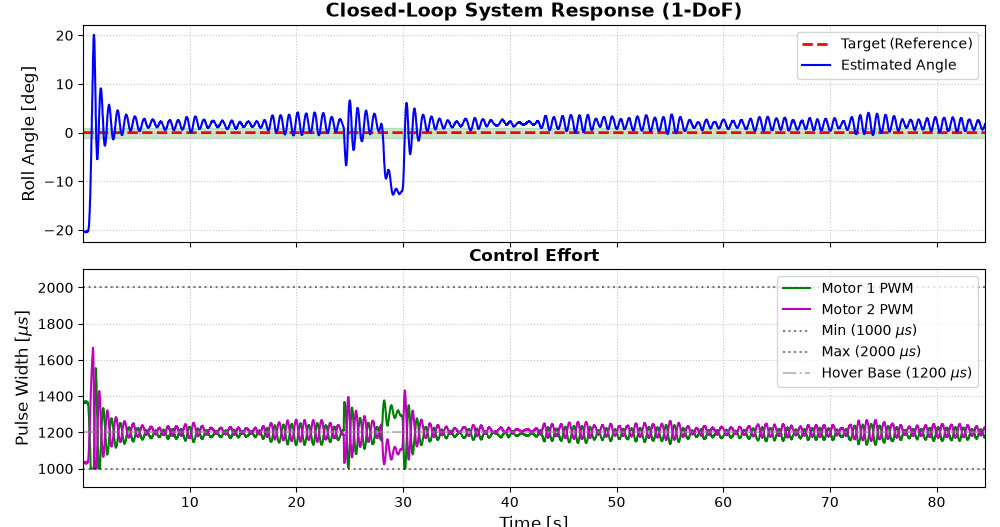
\includegraphics[width=1.0\linewidth]{PD.png}
    \caption{Closed-loop response of the 1-DoF drone using a Proportional-Derivative (PD) controller. The graph highlights the presence of a persistent steady-state error and the inability to fully reject external disturbances.}
    \label{fig:pd_response}
\end{figure}

As shown in the plot, upon arming, the controller generates an asymmetric impulsive thrust (Motor 2 PWM reaching \SI{1700}{\micro\second}) that rapidly drives the attitude toward the reference setpoint, exhibiting a natural initial overshoot. However, at steady state ($t > \SI{10}{\second}$), the theoretical limitation of the PD controller becomes evident: its inability to eliminate steady-state error in the presence of constant disturbances (e.g., slight mass imbalances). The estimated angle settles with a permanent offset from the $0^\circ$ setpoint. 
Applying an impulsive disturbance (around $t = \SI{25}{\second}$) is damped by the derivative action, but the system returns to the pre-existing \textit{steady-state error}.

\subsection{Test 2: Optimized Transient Response (PID Controller)}
In the second experiment, adding the Integral term (PID) resolves the steady-state offset issue.

\begin{figure}[H]
    \centering
    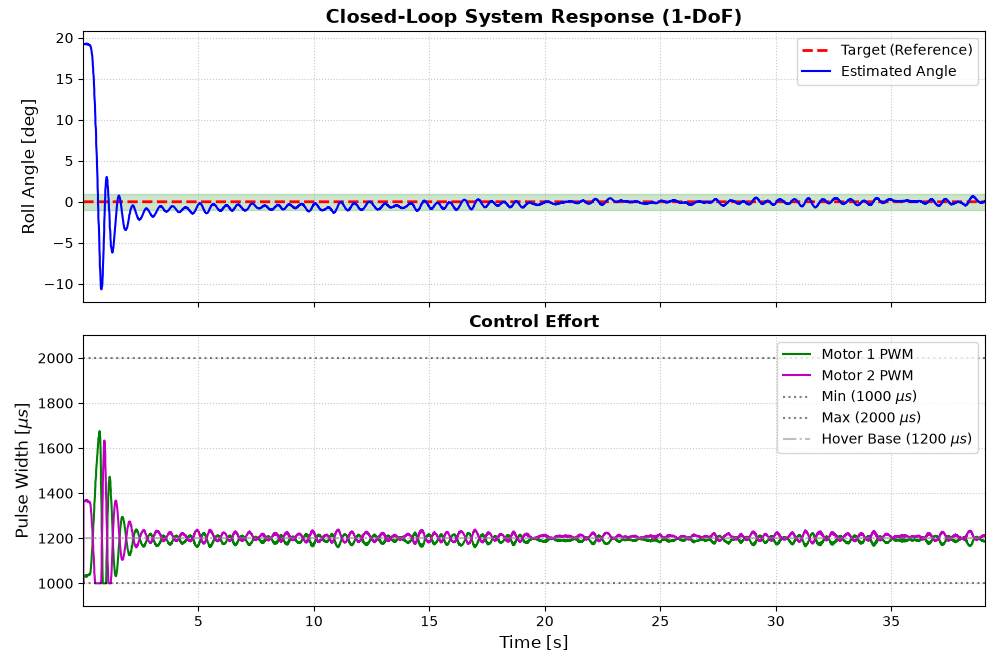
\includegraphics[width=1.0\linewidth]{PID.png}
    \caption{Closed-loop response of the 1-DoF drone using a Proportional-Integral-Derivative (PID) controller.The addition of the integral action successfully eliminates the steady-state offset, allowing the system to accurately maintain the $0^\circ$ setpoint.}
    \label{fig:pid_nodist}
\end{figure}

The step response upon startup exhibits underdamped second-order behavior, with an overshoot of approximately $\pm10^\circ$ damped out within $\sim\SI{3}{\second}$. Once the transient phase concludes, the integral contribution—bounded by the anti-windup algorithm (as described in Section 4.3)—accumulates the residual error and shifts the baseline control effort, completely eliminating steady-state error. From $t = \SI{5}{\second}$ onward, the system holds the reference setpoint within an uncertainty margin of less than $\pm1^\circ$.

\newpage
\subsection{Test 3: External Disturbance Rejection (PID)}
The final test was designed to stress the system at steady state by applying asymmetric physical forces to the drone arm (simulating external wind gusts).

\begin{figure}[H]
    \centering
    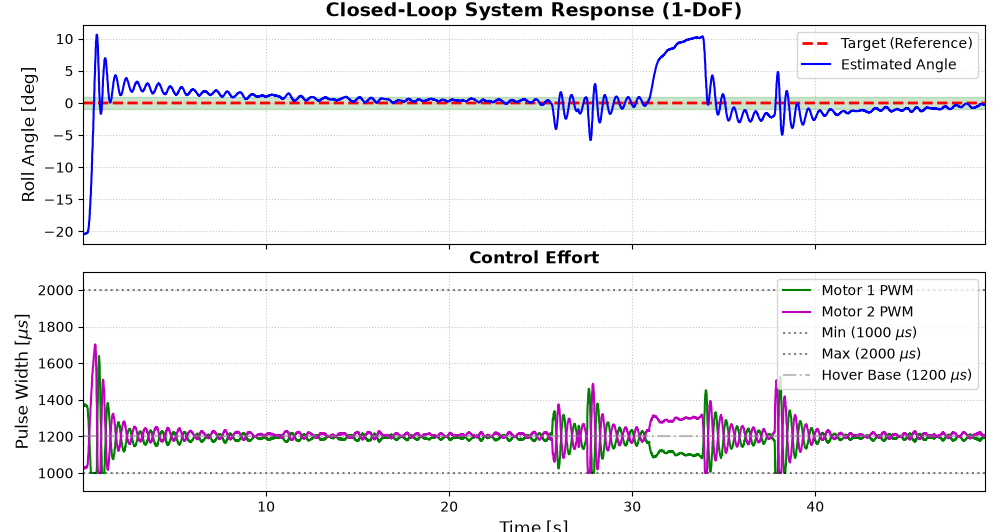
\includegraphics[width=1.0\linewidth]{Disturbi.png}
    \caption{PID controller response to external physical disturbances.}
    \label{fig:pid_disturbances}
\end{figure}

Starting at $t = \SI{25}{\second}$, sequential disturbances are applied. The control effort plot highlights the rapid rejection response: the motors counteract the instantaneous angular rate detected by the gyroscope (via the $K_d$ gain). Specifically, the severe sustained disturbance applied at $t = \SI{31}{\second}$ (forcing the angle up to $+10^\circ$) was fully compensated by the system, which restored equilibrium at $0^\circ$ within roughly $\SI{2}{\second}$ of releasing the external force, without triggering divergent oscillations.

\newpage
\section{Conclusions}
This project successfully validated the synthesis of a digital controller on an ARM Cortex-M4 architecture. Strict timing management via interrupts and DMA proved essential to ensuring accurate execution of the difference equations and complementary filter.

\subsection{Anomaly Resolution: Inertial Reference Drift Upon Reboot}
During experimental testing, an anomalous behavior was observed following warm reboots (Reset): the mechanical range of motion appeared asymmetric in the telemetry interface (e.g., $+25^\circ$ / $-14^\circ$ instead of the nominal $\pm 19^\circ$).

Transient analysis revealed a synchronization issue between mechanical dynamics and firmware calibration. Pressing the Reset button while \textit{hovering} immediately cuts off the PWM signals, causing the drone arm to drop under gravity. However, the microcontroller reboot time is only a few milliseconds, resulting in the immediate execution of the gyroscope offset calibration routine while the arm is still falling. 
Consequently, the firmware sampled the actual angular velocity of the free fall and mistook it for the static \textit{bias} of the inertial sensor. When integrated by the complementary filter, this erroneous offset shifted the logical zero of the system, causing the asymmetric imbalance in the end-stop readings.

The issue was resolved in software by introducing a deterministic \textit{settling time} (\SI{2}{\second}) prior to the calibration routine. This delay, combined with forcing the minimum PWM signal (\SI{1000}{\micro\second}), ensures complete mechanical rest of the structure before measuring the gyroscope's background noise.

\subsection{Parameter Synchronization and Concurrency (Race Conditions)}
Tuning parameters ($K_p$, $K_i$, $K_d$) are received asynchronously via the UART interrupt (handled byte-by-byte at Priority 3). A critical architectural review highlights that transmitting a complete new set of gains simultaneously is not an \textit{atomic} operation.

If the control timer (Priority 1) triggers a PID update mid-way through receiving a burst of serial commands, the controller computes its output using a partially updated state (e.g., new $K_p$ paired with old $K_i$ and $K_d$). This transient parameter inconsistency can induce mechanical jerks or instability in the physical plant for one or more sampling cycles. Furthermore, execution latency in the UART \textit{parsing} routine—if preempted by the high-priority control loop—exposes the peripheral to the risk of a hardware \textit{Overrun Error} (dropped bytes).

\textbf{Future Developments and Mitigation:}
To fundamentally resolve this architectural vulnerability in future iterations, a \textit{Double Buffering} mechanism (\textit{shadow} variables) should be implemented. Incoming serial commands will update only a staging set of temporary variables (e.g., \texttt{Kp\_next}, \texttt{Ki\_next}, \texttt{Kd\_next}). Updating the active PID variables will then occur atomically—in a single block with interrupts disabled (critical section)—exclusively at the start of the subsequent PID cycle or upon receiving an explicit final \textit{commit} command over serial.

\textbf{Additional Future Developments:}
Further enhancements may include transitioning from a single-loop PID controller to a cascaded architecture (outer angle PID loop, inner angular rate PI loop) for even faster disturbance rejection.

\end{document}